\chapter{Implementation} \label{implementation}

For this project I implemented the design as described in the previous chapter.
It is a command line application that takes a source code file as input and
performs semantic analysis on its \gls{ast}. I chose to write my implementation
using the Rust programming language. It is a memory safe language that leverages
the LLVM backend for highly optimized code. This makes it easy to write
robust and performant code. It additionally has very good parallel programming
facilities and an extensive software ecosystem that makes it ideal for this kind
of project. 

\begin{listing}[t]
\begin{minted}[linenos]{text}
fn factorial[n: int] {
    if n == 0 {
        return 1;
    } 

    return (n * factorial(n - 1));
}
\end{minted}
\caption{Factorial in the test language.}
\label{lst:factorial_example}
\end{listing}

Due to a generic lexical and syntatic analysis implementation, as described in the previous chapter,
the compiler supports parsing JSON aswell as a bespoke test language with syntax similar to Rust,
shown in Listing \ref{lst:factorial_example} and \ref{lst:json_example}.

Section \ref{structure} provides an explanation of the programs structure as well as some
implementation details.
\newline \newline
Section \ref{test_lang} discuss the some additional, language specific code that was needed in order
to support \gls{json} and the test langauge.
\newline \newline
Section \ref{dependancies} concludes with a description of the projects dependancies and their
purpose in the implementation.

\section{Structure} \label{structure}

I will explain the implemention in the order of its execution. The program is divided into three
general stages: lexical, syntactic and semantic analysis. Each stage is implemeted just it was
described in the design chapter. There are significant pre-processing steps that need to happen
prior to the core lexing and parsing algorithms, which can be computed at compile time, but I
nevertheless chose to do at runtime. The following section begins by describing this pre-processing
work that initializes key datastructures that are used later in the compiler. The subsequent two
sections describe some implementation details of each of the compilation stages.

\subsection{Lexer Preprocessing} \label{lexer_preprocessing}

In order for the compiler to support different languages, while sharing as much code as possible,
it is neccessary to generate datastructures that can be used by a generic lexer and parser.
Furthermore, the datastructures required for bottom-up parsing are very difficult to create without
some form for automatic generation. Although a hand-written, language specific implementation
has significant optimisation potential, as shown by \cite{langdale_parsing_2019}, the focus of my
implementation is to demonstrate the effectiveness of data-parallel compilation. Single threaded
optimisations that leverage the language or \gls{simd} instructions are sufficiently orthogonal to
this goal to put them outside the scope of the FYP.

In order to for the lexer to work, a state transition table must be obtained. This is done by
reading a file that contains the mapping between the lexemes and their corresponding regular
expressions. An example of the syntax can be seen in listing \ref{lst:json_lexical_grammar}. The
\gls{ast} of each regular expression is then traversed and converted into one, large joint \gls{nfa}
graph using thompson's construction algorithm. This is a classic algorithm that is described by
\cite{aho_compilers_2006}, originally attributed to Ken Thompson. It works by recursively breaking
down the regex into simpler components and building an \gls{nfa} for each component. The resulting
NFA recognizes the same language as the original regex. For my implementation I use an external
library to parse the regex into an \gls{ast}. I then traverse this \gls{ast}, building the \gls{nfa}
as described by the algorithm

This graph is then turned into a \gls{dfa} through powerset construction. For this
algorithm I followed the steps outlined in wikipedia article on powerset construction
\citep{noauthor_powerset_2023}. It works by simulating an \gls{nfa} and interpreting the sets of
states reachable from each state in the \gls{nfa}, as the states of the \gls{dfa}. In other words,
it neccessary to simulate the \gls{nfa} and keep track of all states that the automaton could
reach after seeing an input, according to its nondeterministic choices. Each set of choices is then
converted into a corresponding state in the \gls{dfa}.

An example \gls{nfa} and \gls{dfa} for the JSON grammar is shown in figure \ref{fig:nfa} and figure
\ref{fig:dfa}, respectively. I implemented the graph traversals in both algorithms by keeping track
of a stack of nodes that have already been previously encountered. The \gls{dfa} can be tivially
turned into a state transition table by traversing it from its initial state and  taking note of
each pair of states connected by a transition. The parser similarly requires an operator precedence
table that must be computer generated due to its complexity.

\begin{listing}[t]
\begin{minted}[linenos]{json}
{
  "a": 100,
  "b": {
    "x": [
      100,
      "a"
    ]
  }
}
\end{minted}
\caption{Example of parsable JSON.}
\hrulefill
\label{lst:json_example}
\end{listing}

\subsection{Parser Preprocessing} 

The parser defined by \cite{barenghi_parallel_2015} is a standard operator precedence algorithm that
is modified to allow the parsing of non-terminals. This parser requires that the structure of the
language grammar follow certain rules, as been defined in section \ref{design_parser}. A preliminary
validation of the grammar is performed to ensure that it conforms to these rules. This step also
fixes any production rules with duplicate right-hand sides by creating new production rules with
new non-terminals in a way that keeps the resulting parse tree predictable. After this validation
step, the grammar is ready to be used in the parser. Using this grammar an operator precedence
table can be generated by iterating over the production rules of a grammar in order to determine the
associativity of each terminal symbol.

\subsection{Parallelisation}

Each of the following compilation stages empoly paralleism in the following way. The input into
is first split into equal sized chunks. These chunks are put onto a concurrently accessible work
queue and some number of threads are started. The threads then enter a loop that attempts to take
work from the queue. Once a thread completes processing its work, it makes its results available to
the main thread by storing it in a concurrently accessible skiplist that is common to all threads.
Once all threads terminate, all the work in the workqueue will have been processed with the results
stored in the pre-determined skiplist.

Each thread is initialised with a handle to access the work queue and skiplist, as well as a message
passing channel to communicate with the main thread. If there is no work available, the thread
checks whether it recieved a signal to terminate, otherwise the thread blocks its execution and
waits to be unblocked by the main thread. Once all work on the queue has been processed, the main
thread sends a message to all threads to terminate and unblocks any threads that may have been
blocked. This lifecycle for managing threads ensures that threads don't waste time doing nothing and
are terminated by the program rather than the operating system.

\subsection{Lexical Analysis}

The analysis begins by initialising a lexical analyzer instance for each possible state the input can be in. This set of analyzer instances is executed sequentially on a work thread, one such set per chunk of input. This is because there is no way to tell whether the analysis has begun in the middle of an identifier, string or other multi-character lexeme. The reasons for this are described in the literature review. The set of possible start states have been discovered during the construction of the \gls{dfa}, described in section \ref{lexer_preprocessing}.

\begin{figure}[t]
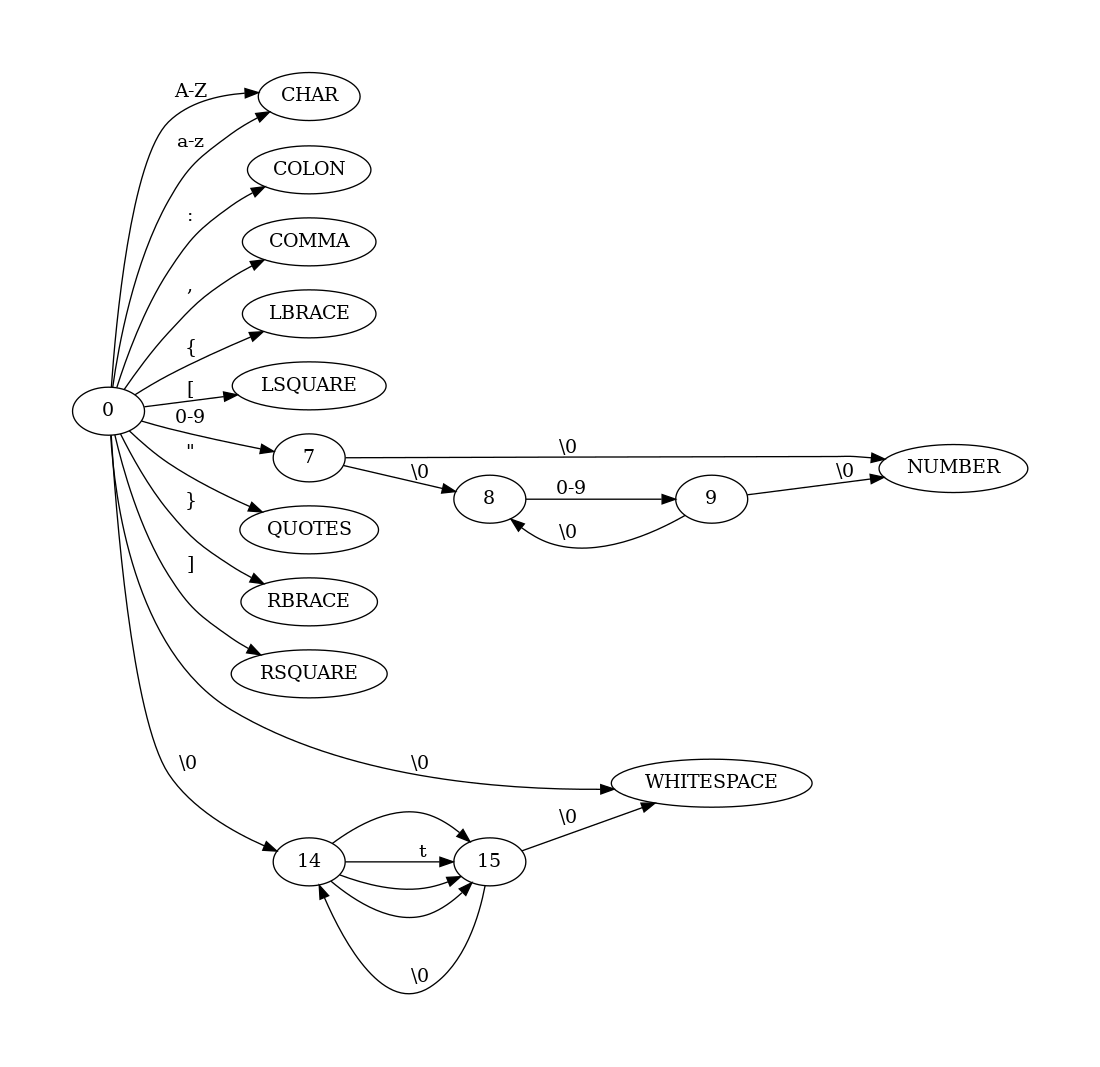
\includegraphics[width=0.8\textwidth]{images/nfa.png}
\caption{NFA of the JSON lexical grammar}
\label{fig:nfa}
\end{figure}

\begin{figure}[t]
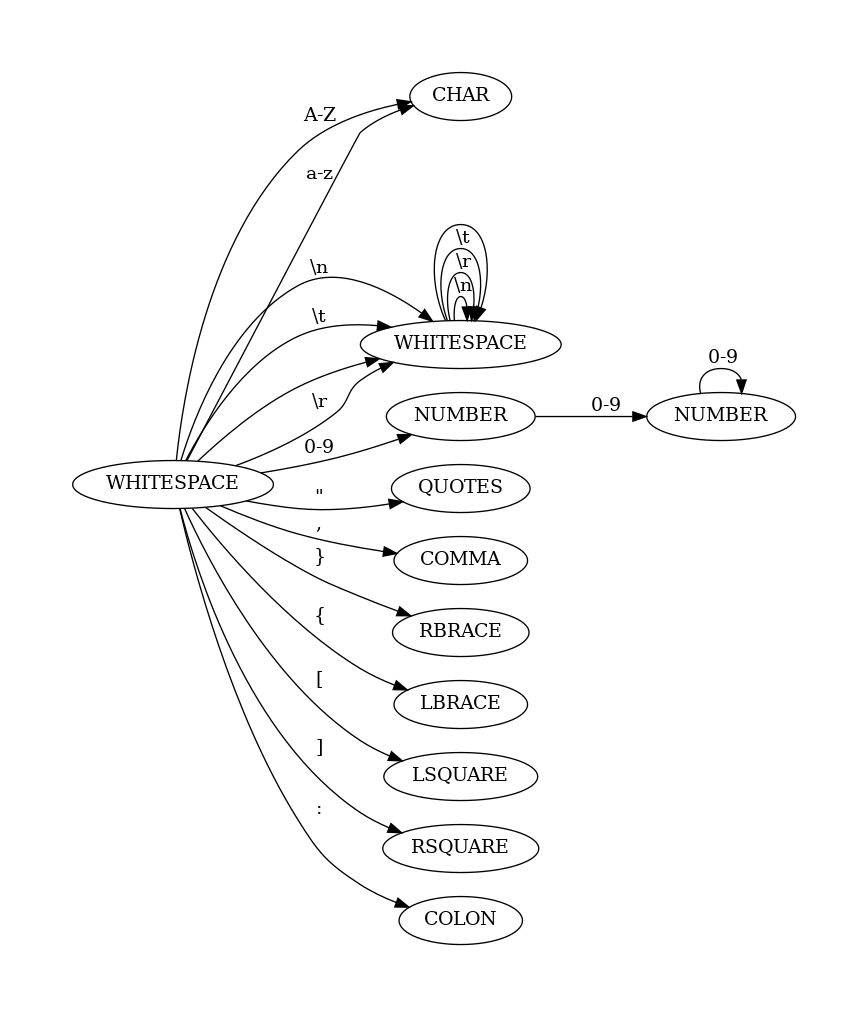
\includegraphics[width=0.8\textwidth]{images/dfa.png}
\caption{DFA of the JSON lexical grammar}
\label{fig:dfa}
\end{figure}

Lexical analysis is performed by processing each character of the input and feeding it into each
lexer instance. Since only the analyzers that begin at a potentially correct start state will
process the input without error, if a lexer instance does encounter an error, it no longer needs
to be processed. 

Each analyzer works by the taking its current state and input symbol and using it to get a new state
from the state transition table. If there is no state for the given state-symbol pair, the instance
checks whether its current state is a terminal state and emits the corresponding lexeme. If there is
not state it can transition to and there is no lexeme to emit, the lexer reaches an error state and
no longer accepts input. 

Once the input has been processed, the outputs from each group lexer instances is placed in the
output skiplist. Once the whole work queue is empty and threads have terminated, the array of
outputs is joined together into one array of lexemes. This is done by iterating over the list and
choosing the outputs that completed analyzing successfully and have the same inital state as the
previous outputs final state. This array of lexemes is then passed onto the syntactic analyzer.

\subsection{Syntactic Analysis}

Syntactic analysis is performed by following the algorithm described in
\cite{barenghi_parallel_2015}. It is a standard  operator precedence parsing algorithm that is
modified to allow for non terminals. Similarly to the lexer, this algorithm requires two passes over
the input. The first pass splits the source string into chunks. Each chunk is assigned to a separate
worker and when all chunks are parsed then the outputs are recombined. Each output consists of a
parse tree, possibly with leading and trailing lexemes that couldn't not be reduced by the parser.
Each two consecutive outputs are then merged such that parsing can continue on the merged whole.
This continues until the parse tree is complete.

\begin{figure}[h]
	\begin{subfigure}[t!]{0.5\textwidth}
	    \centering
	    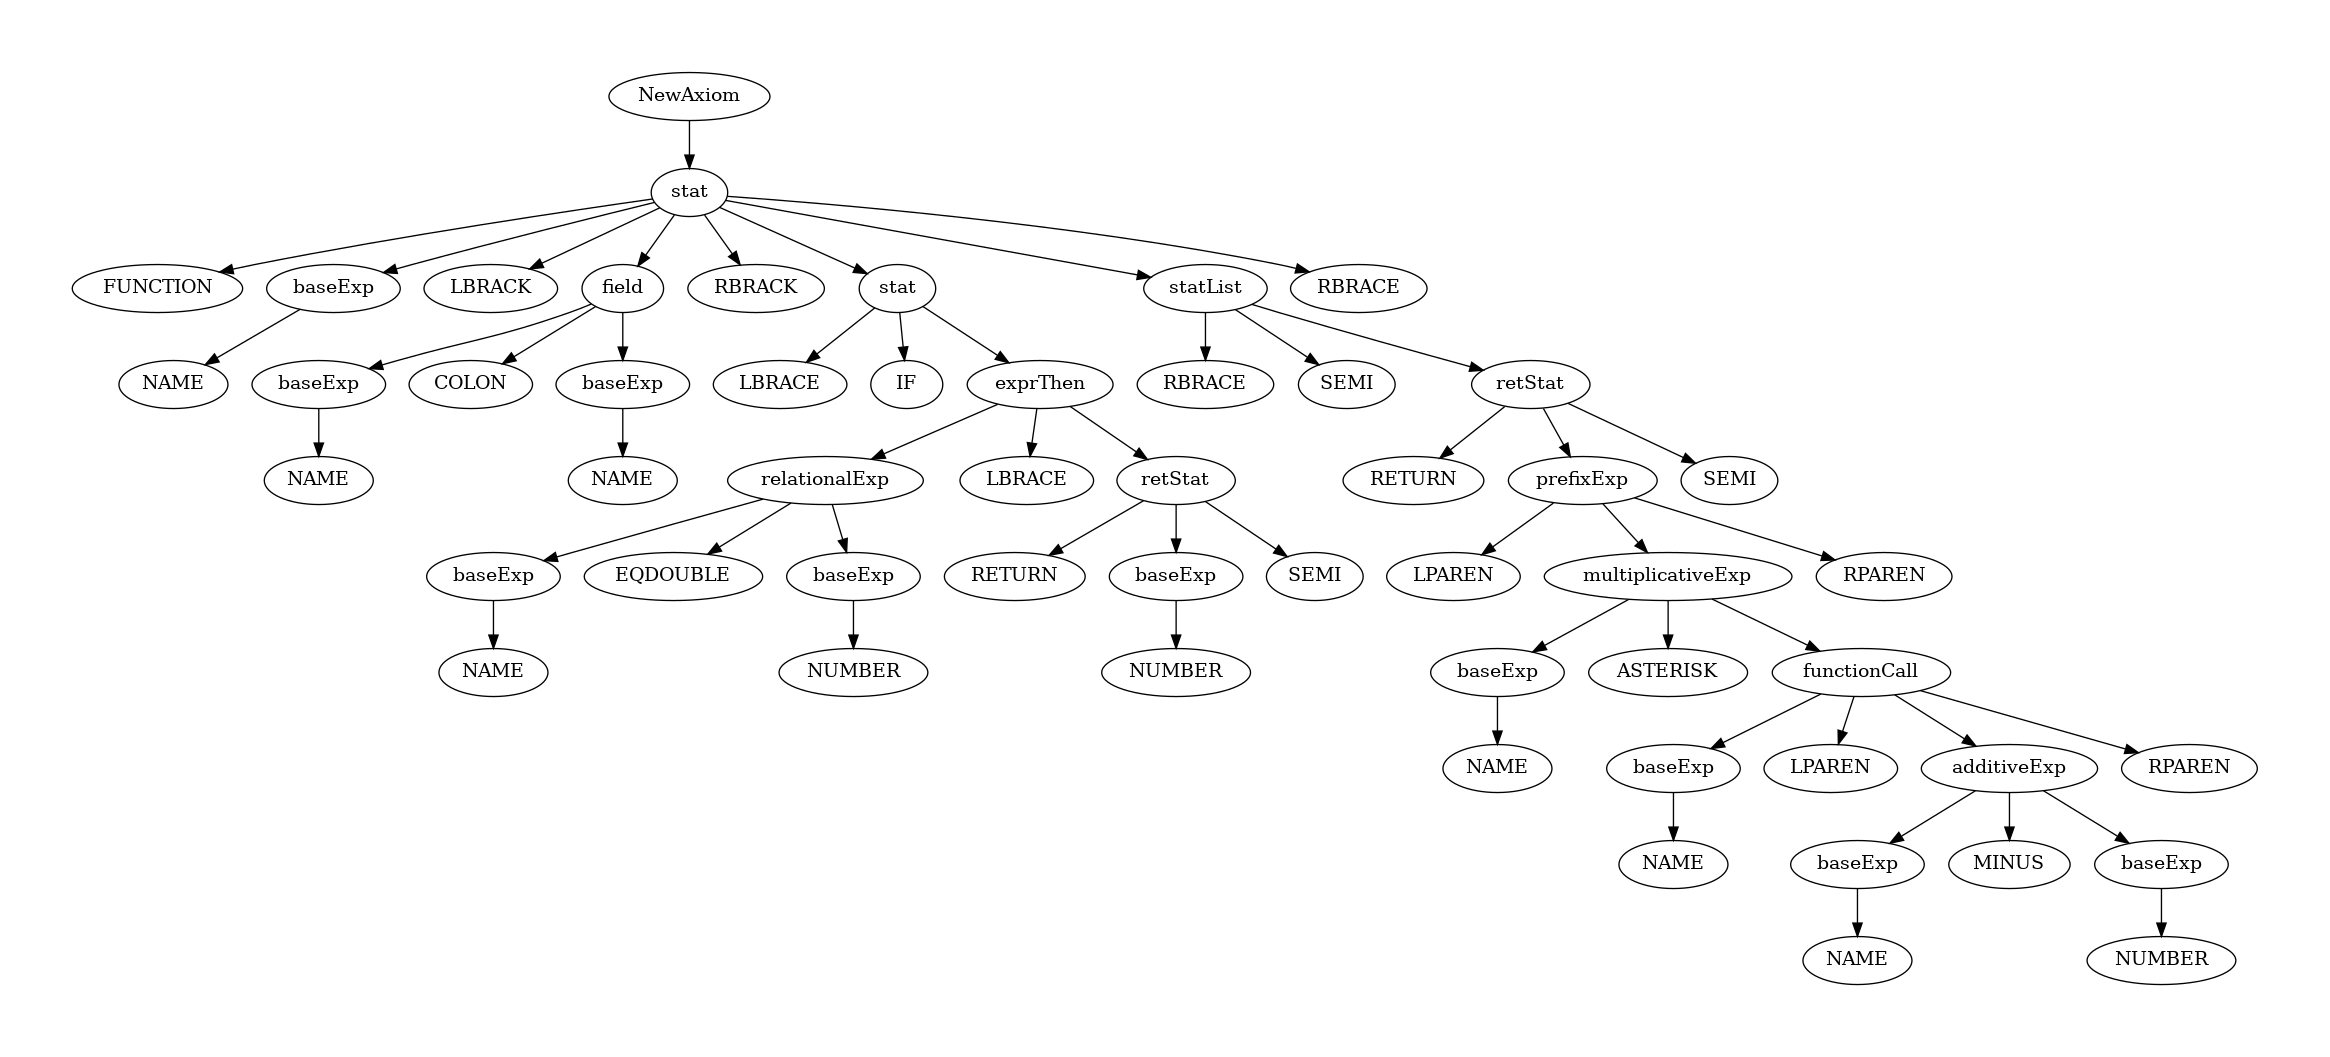
\includegraphics[width=\textwidth]{images/ptree.png}
	\end{subfigure}
	\begin{subfigure}[t!]{0.5\textwidth}
	\centering
	\begin{minted}[breaklines=true, fontsize=\scriptsize]{text}
fn add[a: int, b: int] {
	return a + b;
}
	\end{minted}
	\end{subfigure}%
	\caption{Visualization of the parse tree on the left with the source code on the right. Terminals are capitalised and nonterminals are in camel case.}
	\label{fig:parse_tree}
\end{figure}

\section{Test Langauge Processing} \label{test_lang}

The implementation described thus far can analyse a simple language, such as \gls{json}, without any
modification. All that needs to be specified is a lexing and parsing grammar. This it not the case
with the test langauge due to limitations in the lexing and parsing algorithms.

The syntax of a typical programming language consists of a nested list of statements. Since the
parser requires a terminal between every two non-terminals, any list of of such statements requires
some kind of non-terminal delimeter. A natural choice for this for delimiter is the semicolon
becasue it is also used for this purpose in other programming langauges. An issues arises however
when one considers if, while and function definition statements. Each of these statements unexpectedly requires a semicolon its end. This is very cumbersome and requires that the lexer insert semicolons between pairs , such as between right curly brackets and any lexeme that a statement can begin with.

Another issue I encountered is ditinguising between a unary and binary minus. The parser on
its own is incapable of disovering this distinction because it can potentially lack the context
surrounding a minus lexeme. For example, if the expression $a - b$ were to be parsed starting from
the $-$ symbol, the parser would incorrectly assume that $-$ is a unary operator with $b$ as the
operand. My solution is to emit a different lexeme during lexical analyzer depending on whether any
whitespace was encountered between the a minus sign and the subsequent lexeme.

Due to a limitation of the regular expression parser that is used to read the lexical grammar,
it is not possible to use the look-back regular expression operator. This makes it impossible to
recognise whether an input string is an identifier or a key word of the language in the current
implemetnation. I work around this by defining the keywords separately from the main lexical grammar
and creating a second transtition table from them that is then used to re-analyze any lexemes that
could be a key word of the language.

Semantic analysis of the \gls{ast} checks whether all variables have been used and defined according
to standard scoping rules.

\section{Online Compiler} \label{test_lang}

I decided to create an online compiler demonstration in order to visualize the compiler's outputs
with a graphical user interface. This was made possible by the Rust compiler's ability to compile
code into web assembly. The online compiler executes entirely client side without the need to run
code on a remote server. Webassembly lacks multi-threading capabilities and as such
the demonstration is entirely single threaded.

\section{Dependencies} \label{dependancies}

Code dependencies in the Rust code ecosystem that are  available through the cargo package manager
are called crates. These crates are comparable to small, open source, third party libraries that can
easily be integrated into a rust project. In this section I mention the code dependencies I've used
in my implementation in order to illustrate what parts of my project were accomplished through the
use of third party code.

\subsection{Core}

\textbf{crossbeam} - Common data structures for implementing parallel systems.
This crate implements a concurrently accessible queue, skiplist and a
multi-producer, multi-consumer message passing channel. All of these data
structures are important for reliably sharing data across threads.
\newline\newline
\textbf{regex-syntax} - A crate for parsing standard regular expression syntax.
It provides a simple \gls{ast} that the lexer uses to read the mappings from
lexemes to regular expression patterns.
\newline\newline
\textbf{dot} - A crate that makes it easier to generate graphs in the dot
language. Its used to visualise the parse tree and \gls{ast}.
\gls{ast}.
\newline\newline
\textbf{criterion} - Reliable benchmarking facilities for testing the performance of the
compiler with differently sized inputs.

\subsection{Utility or Minor Contribution}
\textbf{tinyrand} - A lightweight implementation of random number
generation. It is used for creating unique IDs for bathes of work in the work
queue.
\textbf{serde} - Serialization and deserialization capabilities for transferring
code to and from the javascript runtime when running in the browser.
\newline\newline
\textbf{wasm-bindgen} - Macro's for easily creating bindings to javascript when
compiling to web assembly.
\newline\newline
\textbf{log, flexi\_logger ,wasm\-logger, console\_error\_panic\_hook} - Various
crates for logging to files as well as to the terminal, improved formatting and
correct logging when running in the browser.
\newline\newline
\textbf{simple-error} - A simple library for creating errors from error messages
instead of creating types for every error.

\subsection{Optimisation}
\textbf{memmap} - An interface for using linux's memmap syscall. Using memap to
read large files is  faster than using the standard read syscall.
\newline\newline
\textbf{bittyset} - A set implementation that uses a bit vector as a backing
store. This enables a compact representation as well as faster set operations in
the parser where sets of terminals and non-terminals are used.


